En esta sección se realizará una primera aproximación a la posible interfaz que tendrá el portal, detallando y explicando las vistas que la conforman.  A continuación se mostrarán los \textit{mockups} de la interfaz y se explicará cada uno de ellos.



\subsection{Interfaz de la zona de datos}
Como se ha mencionado en la sección ``\nameref{definicion_sistema}'' perteneciente al capítulo \ref{chapter04}, la interfaz de zona de datos (o \textit{LandBook}) queda fuera del alcance de éste proyecto, por lo que no se mostrarán \textit{mockups} para dicha sección.



\subsection{Interfaz de administración}
La interfaz de administración será directamente proveída por el gestor de contenidos que, como se ha mencionado en la sección ``\nameref{chapter02:alternativas_seleccionadas}'' perteneciente al capítulo \ref{chapter02}, será Drupal.  Por esta razón no se mostrarán \textit{mockups} pertenecientes a dicha interfaz.



\subsection{Interfaz de la zona social}
A continuación se mostrarán los \textit{mockups} de la zona social (o \textit{LandDebate}).


\subsubsection{Vista del blog del Land Portal}
\label{chapter04:mockup_blog}
La figura \ref{fig:mockup_blog} muestra el \textit{mockup} de la vista que conformará el blog del nuevo Land Portal.

Ésta pantalla mostrará las entradas del blog ordenadas de más a menos reciente.  Las tres entradas más recientes se destacarán sobre el resto, e incluirán:
\begin{itemize}
	\item Título de la entrada, enlazado a la vista de detalle de la propia entrada.
	\item Imagen de la entrada.
	\item Autor y fecha en la que la entrada fue añadida al blog.
	\item Tópicos relacionados.  Al pulsar en un tópico, se accederá a una vista en la que se mostrarán todos los contenidos del portal relacionados con dicho tópico.
	\item Resumen del contenido de la entrada.
\end{itemize}

\begin{figure}[h]
	\centering
	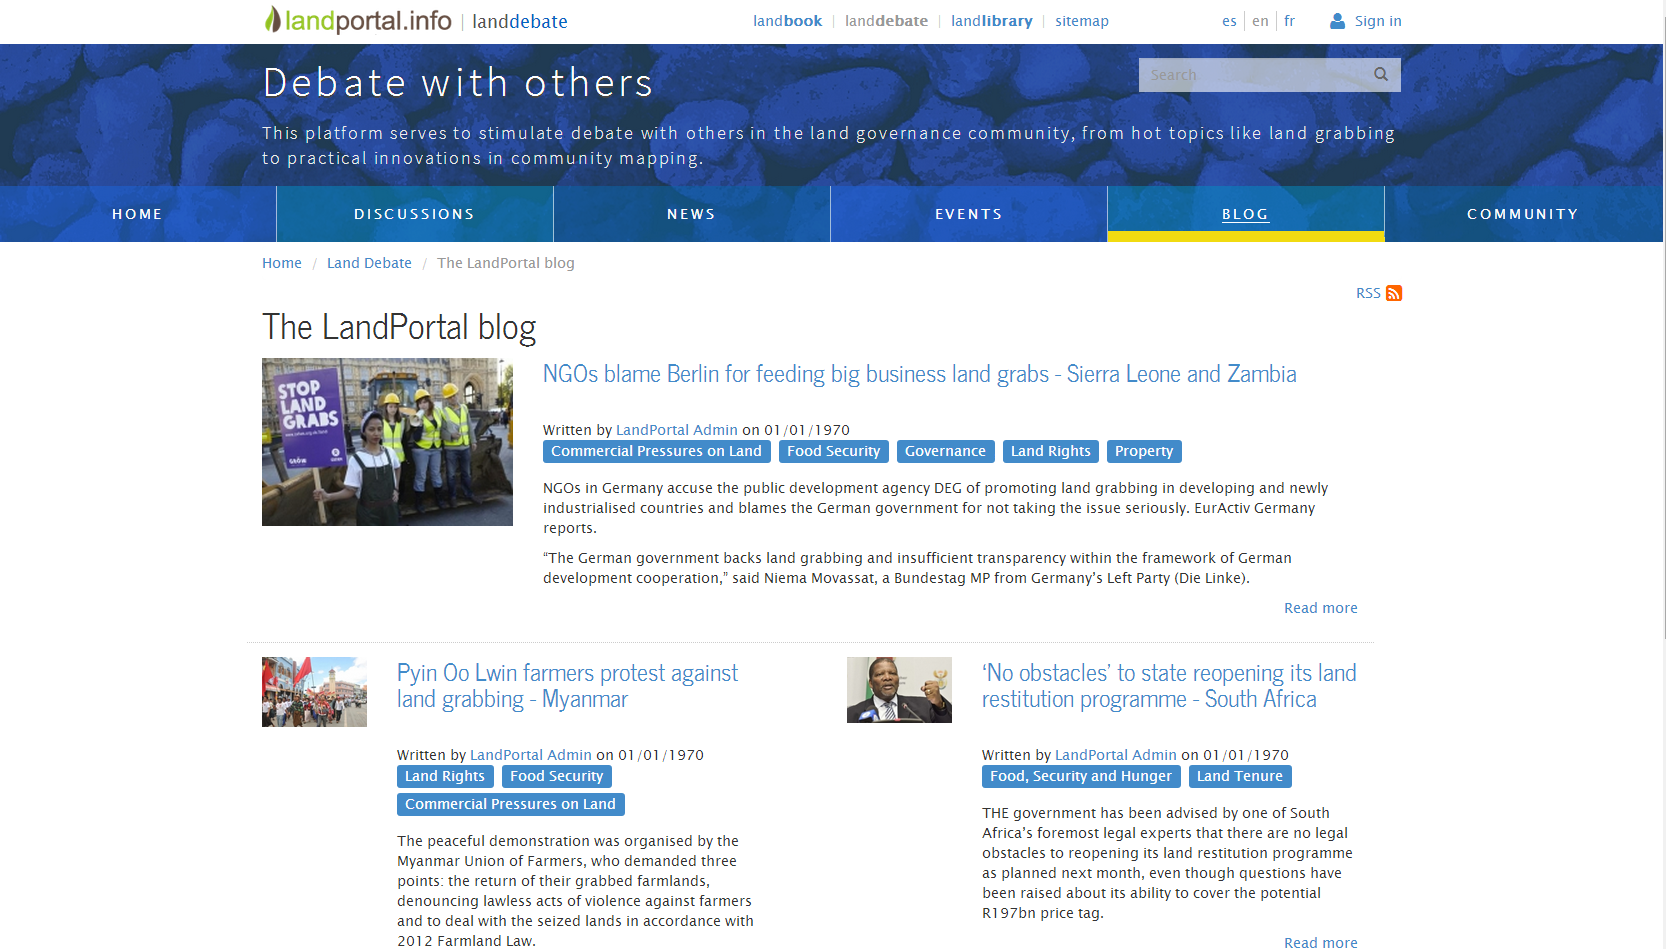
\includegraphics[width=\textwidth]{mockups/blog}
	\caption{\textit{Mockup} de la vista del blog del Land Portal}
	\label{fig:mockup_blog}
\end{figure}

Las entradas anteriores tendrán menos énfasis en la vista, y sólo estarán representadas por su título y la fecha en la que han sido creadas.  Además también se incluirá un paginador para recorrer las noticias anteriores y un enlace al \textit{feed} RSS\footnote{El feed RSS permite suscribirse a las últimas entradas del blog utilizando un lector de feeds RSS como Feedly, Newsvibe o Digg Reader y obtener las actualizaciones de forma automática en el lector sin necesidad de acceder al portal.} donde también se encontrarán las últimas noticias.


\subsubsection{Vista de detalle de una entrada del blog}
\label{chapter04:mockup_blog_entry}
La figura \ref{fig:mockup_entrada_blog} muestra el \textit{mockup} de la vista de detalle de una entrada del blog.  Esta vista incluirá:
\begin{itemize}
	\item Título de la entrada
	\item Autor y fecha de creación de la entrada
	\item Tópicos relacionados.  Como ya se ha explicado anteriormente, al pulsar sobre un tópico, el sistema cargará una vista con todos los contenidos relacionados con dicho tópico.
	\item Contenido de la entrada
	\item Imagen relacionada
	\item Botones destinados a compartir el contenido de la entrada en redes sociales como Twitter o Facebook.
\end{itemize}

En la zona inferior de la vista se incluirá la sección de comentarios.  En esta sección los usuarios podrán participar y dar su opinión a cerca del tema tratado en la entrada del blog.  Cada comentario mostrará su contenido, su autor y la fecha en al que fue creado.  Los comentarios se mostrarán ordenados según su fecha de creación.

\begin{figure}[h]
	\centering
	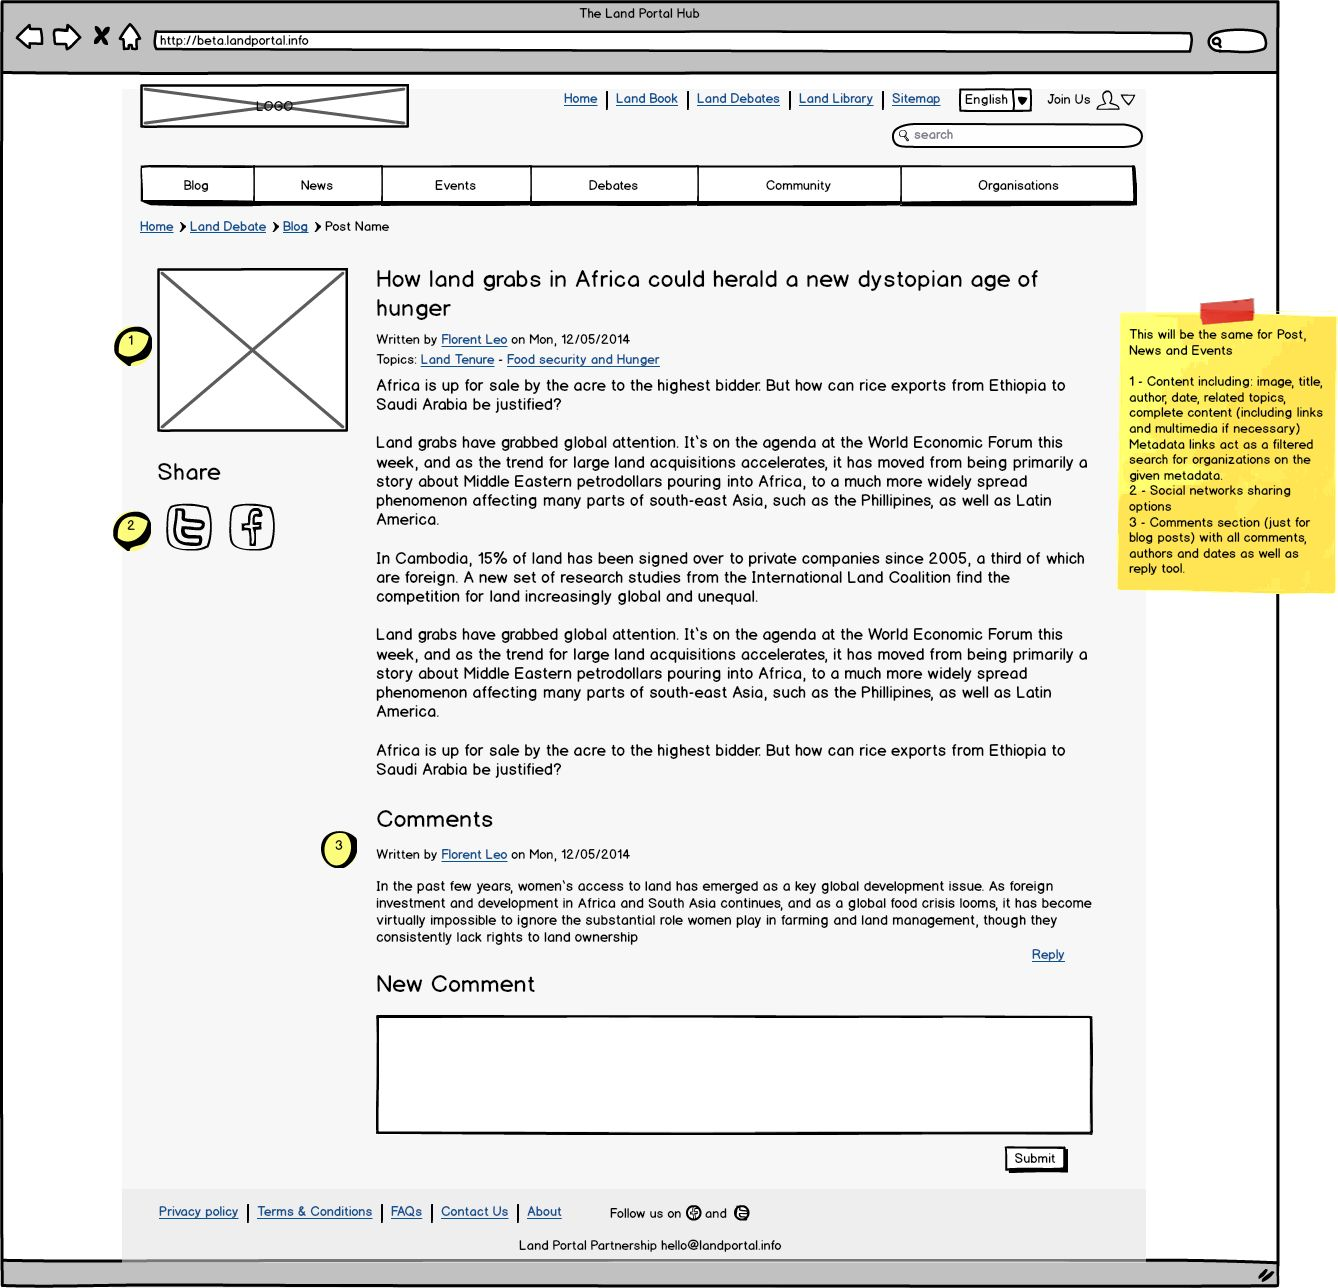
\includegraphics[width=\textwidth]{mockups/post-new-event}
	\caption{\textit{Mockup} de la vista de detalle de una entrada del blog}
	\label{fig:mockup_entrada_blog}
\end{figure}


\subsubsection{Vista de eventos}
\label{chapter04:mockup_eventos}
La figura \ref{fig:mockup_eventos} muestra el \textit{mockup} de la vista de eventos del nuevo Land Portal.  Los dos eventos más recientes se destacarán sobre el resto e incluirán:
\begin{itemize}
	\item Título del evento, enlazado a la vista de detalle del propio evento.
	\item Imagen del evento.
	\item Autor y fecha en la que el evento fue creado.
	\item Tópicos relacionados.  Al pulsar en un tópico, se accederá a una vista en la que se mostrarán todos los contenidos del portal relacionados con dicho tópico.
	\item Resumen del contenido del evento.
\end{itemize}
De forma similar a como sucede en el blog, los eventos anteriores tendrán menos importancia en la vista, y únicamente se mostrarán con su título y la fecha en la que el evento tiene lugar.  También al igual que el blog, se incluye un paginador y un enlace al \textit{feed} RSS donde también se encontrarán los últimos eventos.

Un añadido especial de ésta vista es un calendario que mostrará resaltados los días en los que tiene lugar algún evento.
\begin{figure}[h]
	\centering
	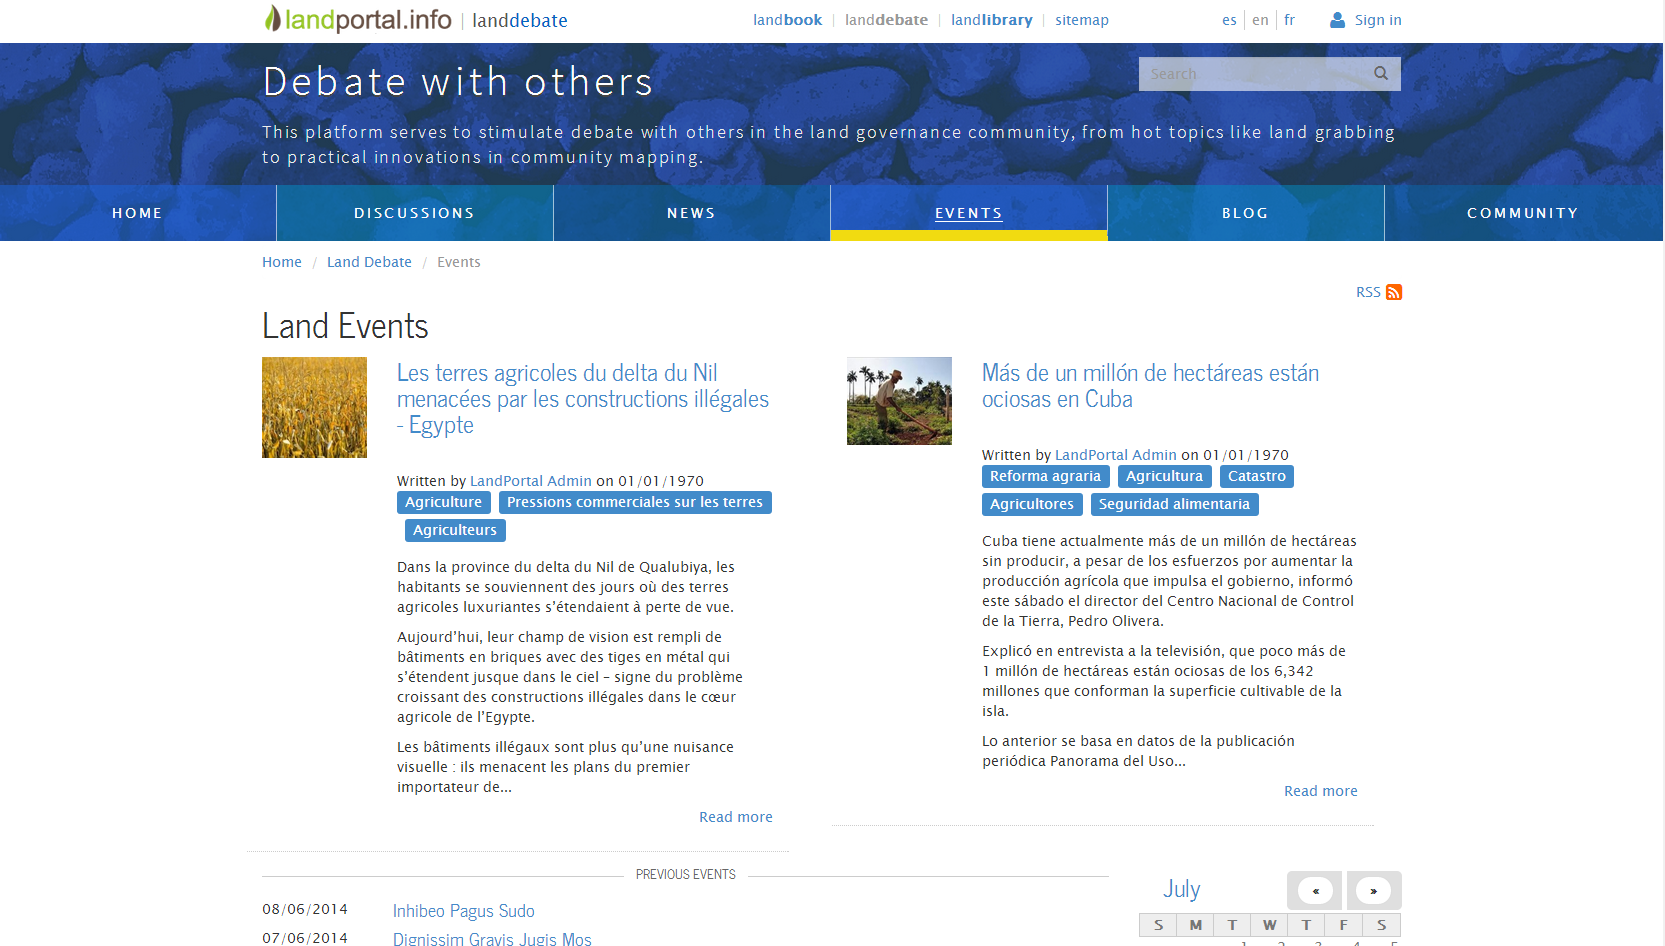
\includegraphics[width=\textwidth]{mockups/events}
	\caption{\textit{Mockup} de la vista de eventos}
	\label{fig:mockup_eventos}
\end{figure}


\subsubsection{Vista de noticias}
\label{chapter04:mockup_noticias}
La figura \ref{fig:mockup_noticias} muestra el \textit{mockup} de la vista de noticias del nuevo Land Portal.  Las cuatro noticias más recientes se destacarán sobre el resto e incluirán:
\begin{itemize}
	\item Título de la noticia, enlazado a la vista de detalle de la propia noticia.
	\item Imagen de la noticia
	\item Resumen del contenido de la noticia.
\end{itemize}
Al igual que en la vista de eventos y del blog, las noticias anteriores sólo mostrarán su título y fecha de creación.  También se incluirán, de la misma forma que las vistas anteriores, un paginador y un enlace al \textit{feed} RSS con las últimas noticias.

Una característica especial de ésta vista será que en la parte izquierda de la misma se mostrarán las últimas actualizaciones de la cuenta de Twitter de Land Portal\footnote{La cuenta oficial de Land Portal se puede ver en \url{https://twitter.com/landportal}}.  Para incluír éste componente se utilizará la capacidad de generación de \textit{widgets} de Twitter.
\begin{figure}[h]
	\centering
	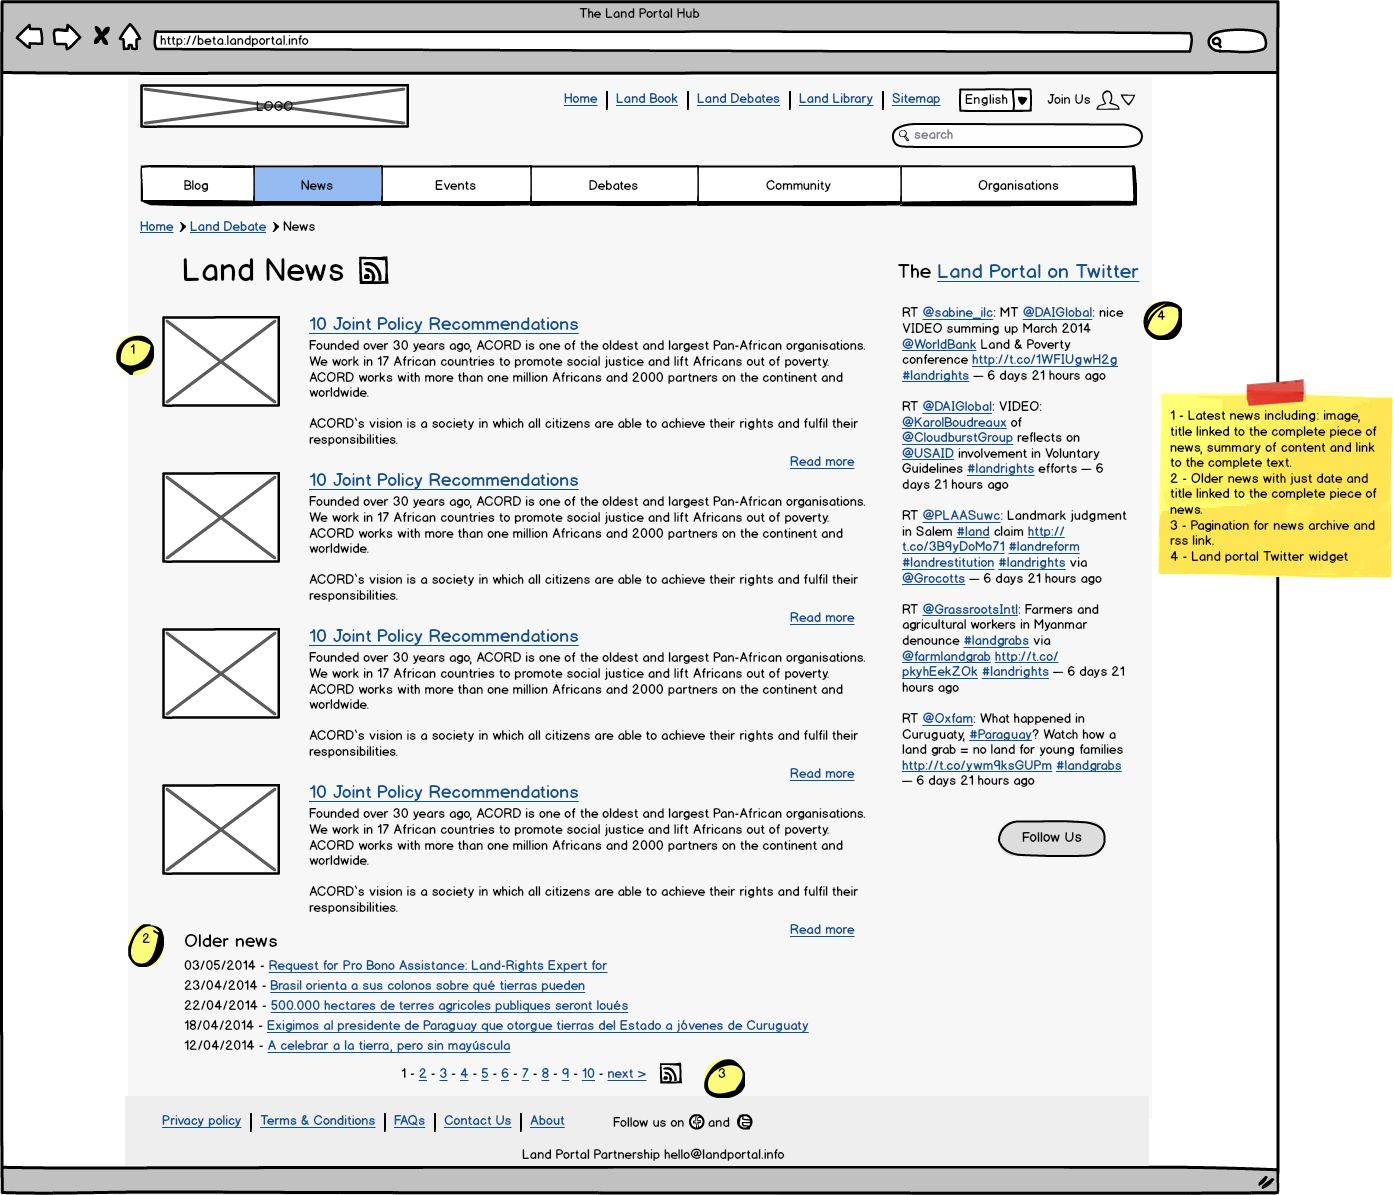
\includegraphics[width=\textwidth]{mockups/news}
	\caption{\textit{Mockup} de la vista de noticias}
	\label{fig:mockup_noticias}
\end{figure}


\subsubsection{Vista de debates}
La figura \ref{fig:mockup_debates} muestra el \textit{mockup} de la vista de debates del nuevo Land Portal.  Ésta vista tiene una importancia clave dentro de la zona social, puesto que los debates serán el principal punto en el que los usuarios participen e intercambien opiniones.  Los debates que no estén cerrados se destacarán sobre el resto e incluirán:
\begin{itemize}
	\item Título del debate, enlazado a la vista de detalle del mismo.
	\item Autor del debate.
	\item Tópicos relacionados.  Al pulsar en un tópico, se accederá a una vista en la que se mostrarán todos los contenidos del portal relacionados con dicho tópico.
	\item Resumen del contenido del debate.
	\item Imagen del debate.
	\item Fecha o fechas en las que el debate tendrá lugar.
	\item Estado del debate.
\end{itemize}

De forma similar a las vistas anteriores, también se incluirán los debates anteriores (en este caso los debates ya cerrados) únicamente con su título y la fecha en la qu ese han creado y un enlace al \textit{feed} RSS de la sección de debates.

Puesto que, como se ha dicho anteriormente, ésta vista juega un papel clave fomentando la participación de los usuarios en el portal.  Por ello, en la zona derecha se mostrarán los últimos comentarios que los usuarios hayan realizado en algún debate.  Cada comentario incluirá:
\begin{itemize}
	\item Fecha de creación del comentario.
	\item Autor del comentario.
	\item Título del comentario enlazado al propio comentario dentro de la vista de detalle del debate.
	\item Resumen del contenido del comentario.
\end{itemize}
\begin{figure}[h]
	\centering
	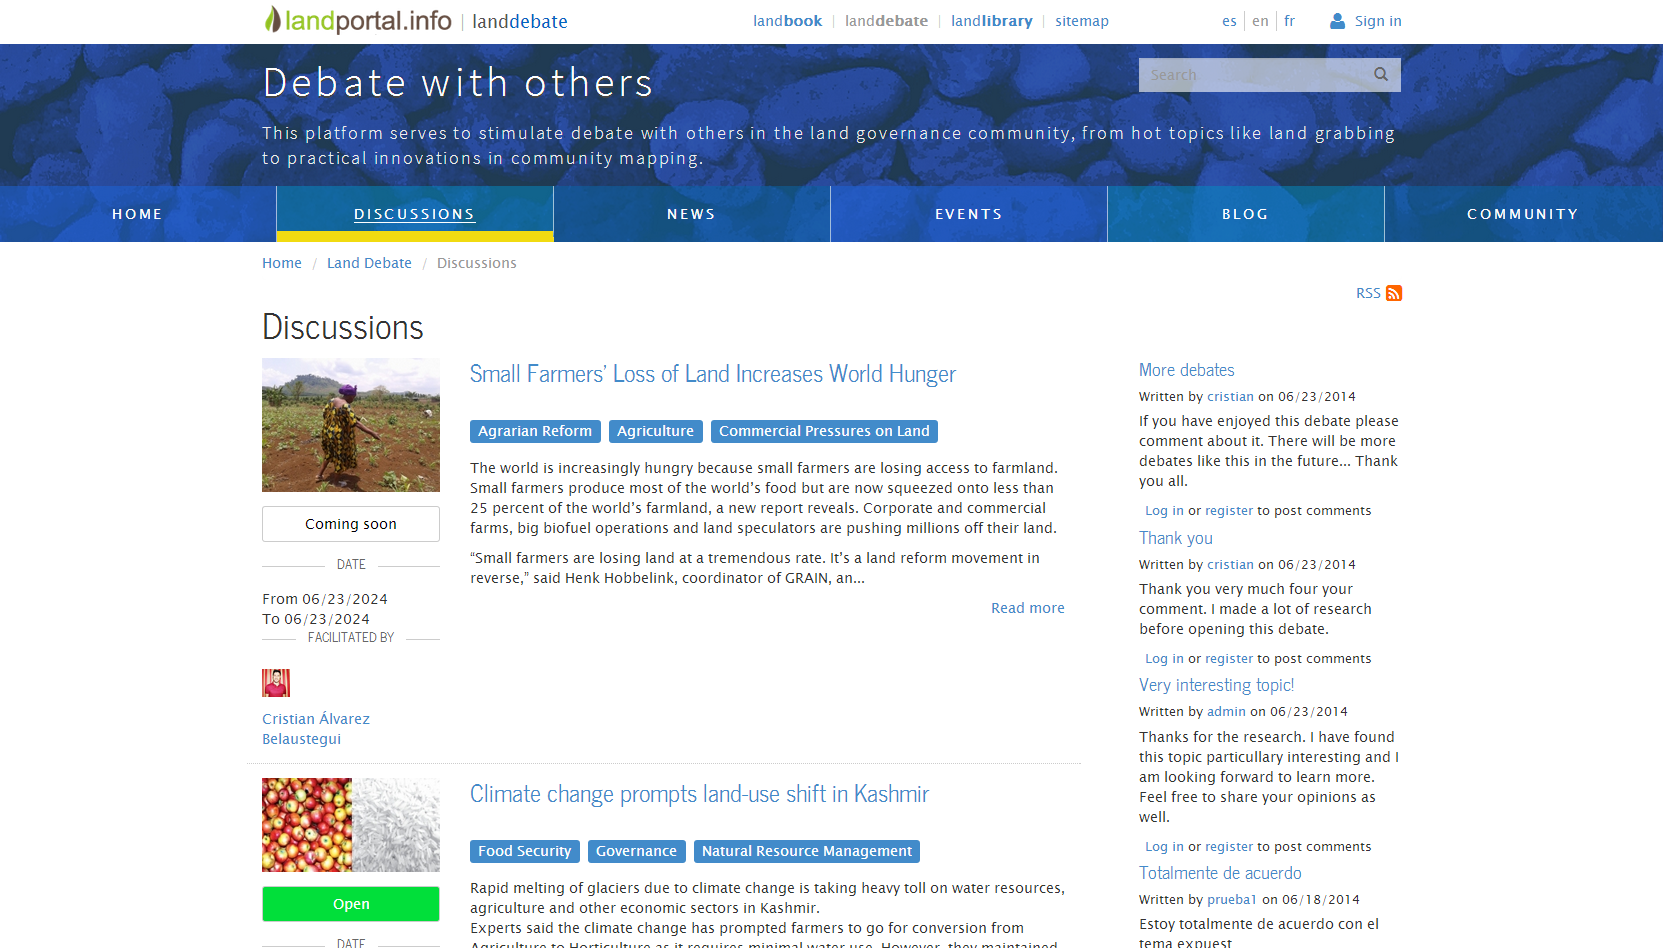
\includegraphics[width=\textwidth]{mockups/debates}
	\caption{\textit{Mockup} de la vista de debates}
	\label{fig:mockup_debates}
\end{figure}


\subsubsection{Vista de detalle de un debate}
La figura \ref{fig:mockup_debate} muestra el \textit{mockup} de la vista de detalle de un debate.  Al igual que la vista de debates descrita anteriormente, esta vista juega también un rol clave para fomentar la participación de los usuarios en el portal.

La vista incluirá toda la información del debate, incluyendo:
\begin{itemize}
	\item Título del debate
	\item Tópicos y países relacionados
	\item Idioma en el que tendrá lugar el debate
	\item Contenido del debate
	\item Imagen del debate
	\item Estado
	\item Autor del debate
\end{itemize}

En la parte inferior de esta vista se ubicará la sección de comentarios.  El comportamiento de la sección de comentarios variará en función del estado del debate.  Cuando el debate esté abierto, los usuarios podrán participar e incluir nuevos comentarios o  responder a los comentarios ya existentes.  Cuando el debate esté cerrado se mostrarán los comentarios existentes, pero no se permitirá añadir ningún comentario nuevo.  Los comentarios se mostrarán ordenados según su fecha de creación.

Para reforzar la función social de esta vista, se incluirán también una serie de botones que permitirán compartir el debate en redes sociales como Twitter o Facebook.  Al mismo tiempo, en la parte derecha de la vista se mostrarán los últimos comentarios relacionados en la red social Twitter.

\begin{figure}[h]
	\centering
	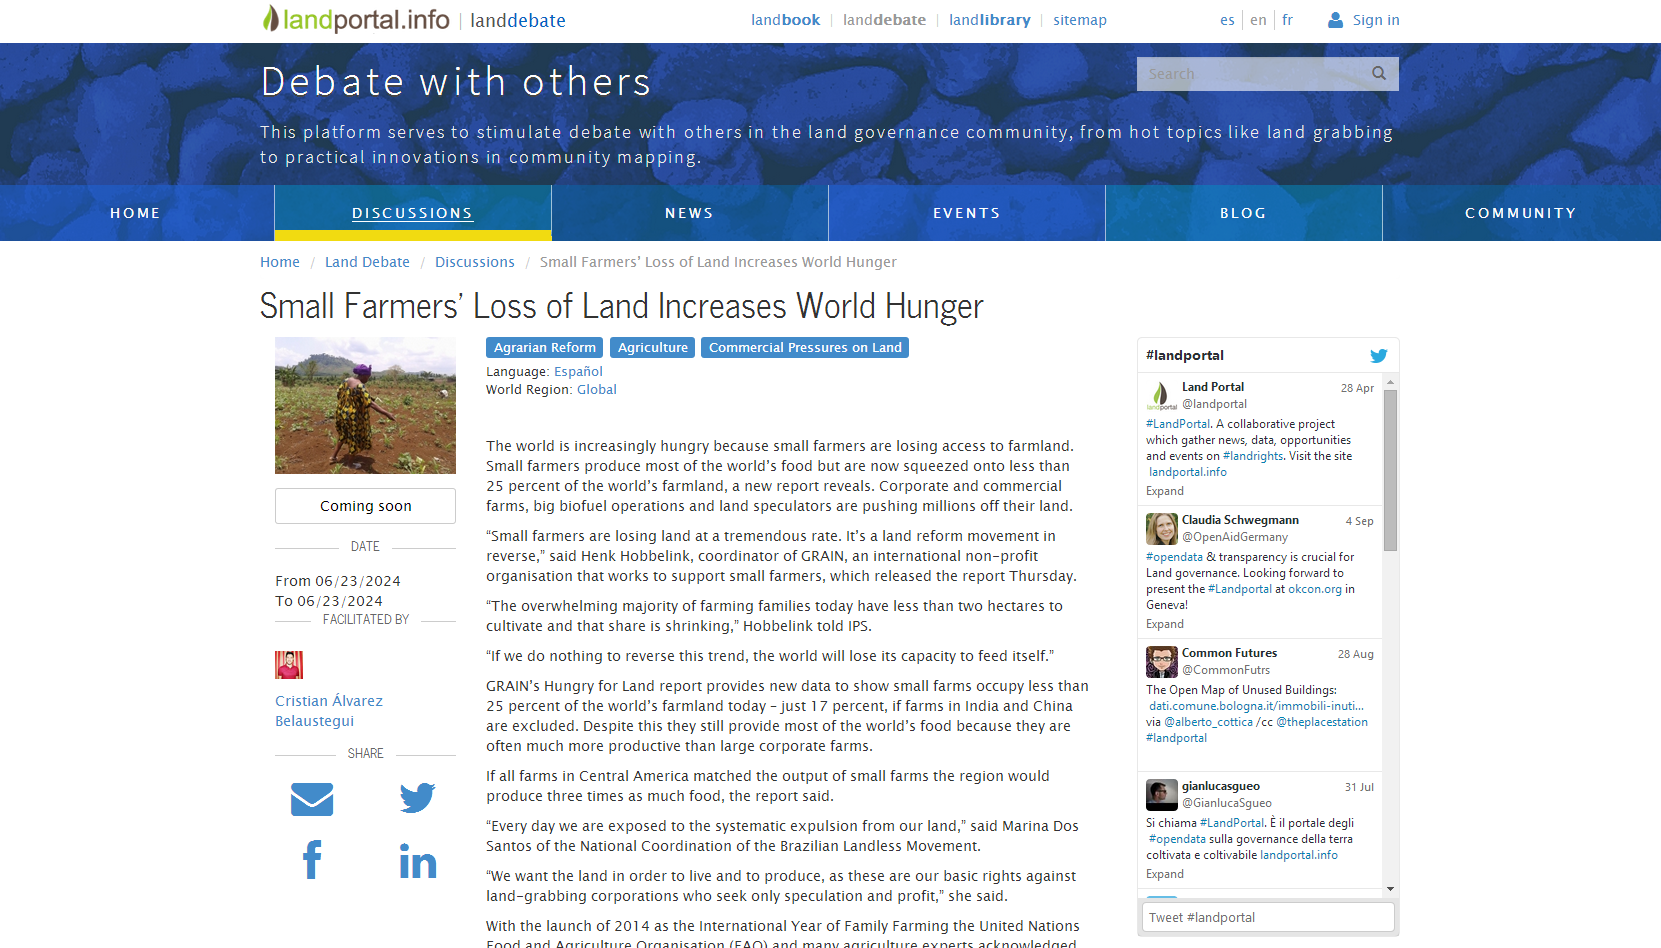
\includegraphics[width=\textwidth]{mockups/debate}
	\caption{\textit{Mockup} de la vista de detalle de un debate}
	\label{fig:mockup_debate}
\end{figure}


\subsubsection{Vista de detalle de un evento y de una noticia}
\label{mockup_noticia_evento}
Las vistas del detalle de un evento y una noticia serán similares a la vista de detalle de una entrada en el blog, el \textit{mockup} para dicha vista puede verse en la figura \ref{fig:mockup_entrada_blog}.

La única diferencia de estas vistas respecto a la vista de detalle de una entrada del blog será que ni los eventos ni las noticias tendrán sección de comentarios.


\subsubsection{Vista de organizaciones}
La figura \ref{fig:mockup_organizaciones} muestra el \textit{mockup} de la vista de organizaciones. Esta vista mostrará las organizaciones existentes en el portal en forma de parrilla o \textit{grid}, en la que cada organización mostrará su imagen y su nombre, ambos enlazados a la vista de detalle de dicha organización.

En la zona derecha de la vista se incluirán una serie de controles con los que será posible buscar organizaciones determinadas.  Además, siguiendo con la tónica social del portal ya mencionada anteriormente, se mostrará un \textit{widget} con el contenido de la comunidad de Land Portal en la red social Facebook\footnote{La página oficial de Land Portal en Facebook puede verse en la siguiente dirección: \url{https://www.facebook.com/landportal}}.

\begin{figure}[h]
	\centering
	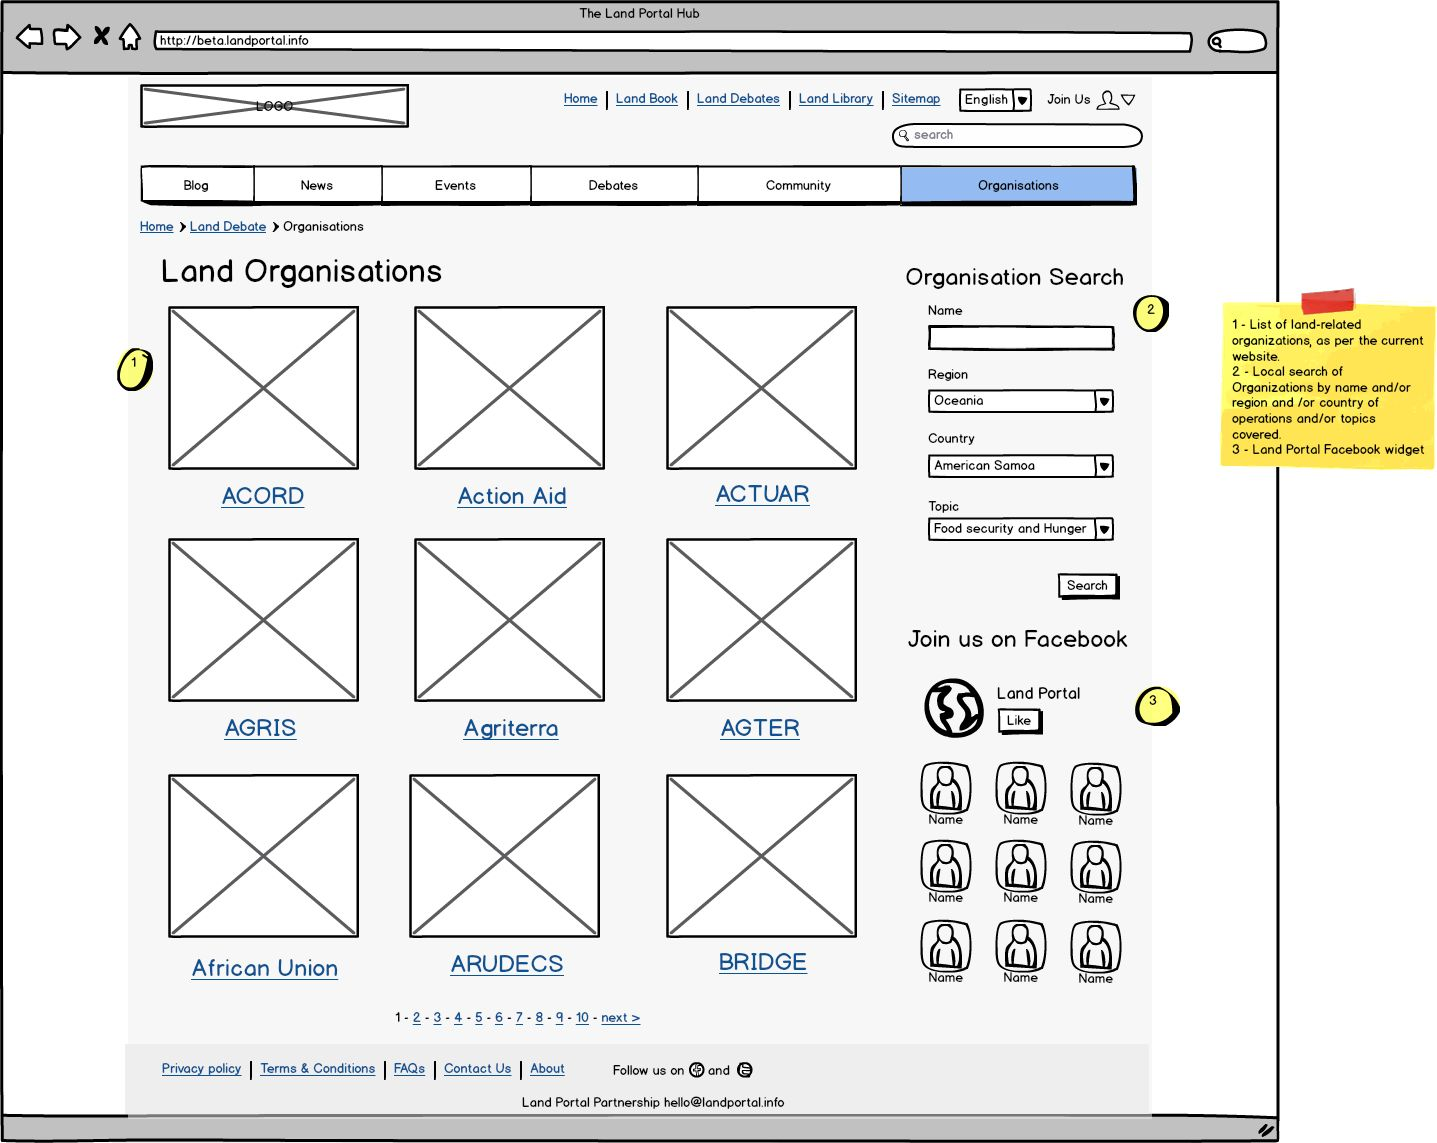
\includegraphics[width=\textwidth]{mockups/organisations}
	\caption{\textit{Mockup} de la vista de organizaciones}
	\label{fig:mockup_organizaciones}
\end{figure}


\subsubsection{Vista de detalle de una organización}
La figura \ref{fig:mockup_organizacion} muestra el \textit{mockup} de la vista de detalle de una organización. Esta vista mostrará las organizaciones existentes en el portal en forma de parrilla o \textit{grid}, en la que cada organización mostrará su imagen y su nombre, ambos enlazados a la vista de detalle de dicha organización.

Esta vista mostrará la imagen, el nombre y una descripción de la organización.  Además también se incluirá un enlace a la página web de dicha organización.  En la parte derecha de la vista se mostrarán los metadatos de la organización, como: el área y los países en los que opera o los tópicos relacionados.  Al pulsar en cualquier término de estos metadatos el sistema cargará una vista que mostrará todo el contenido del portal relacionado con dicho término.

\begin{figure}[h]
	\centering
	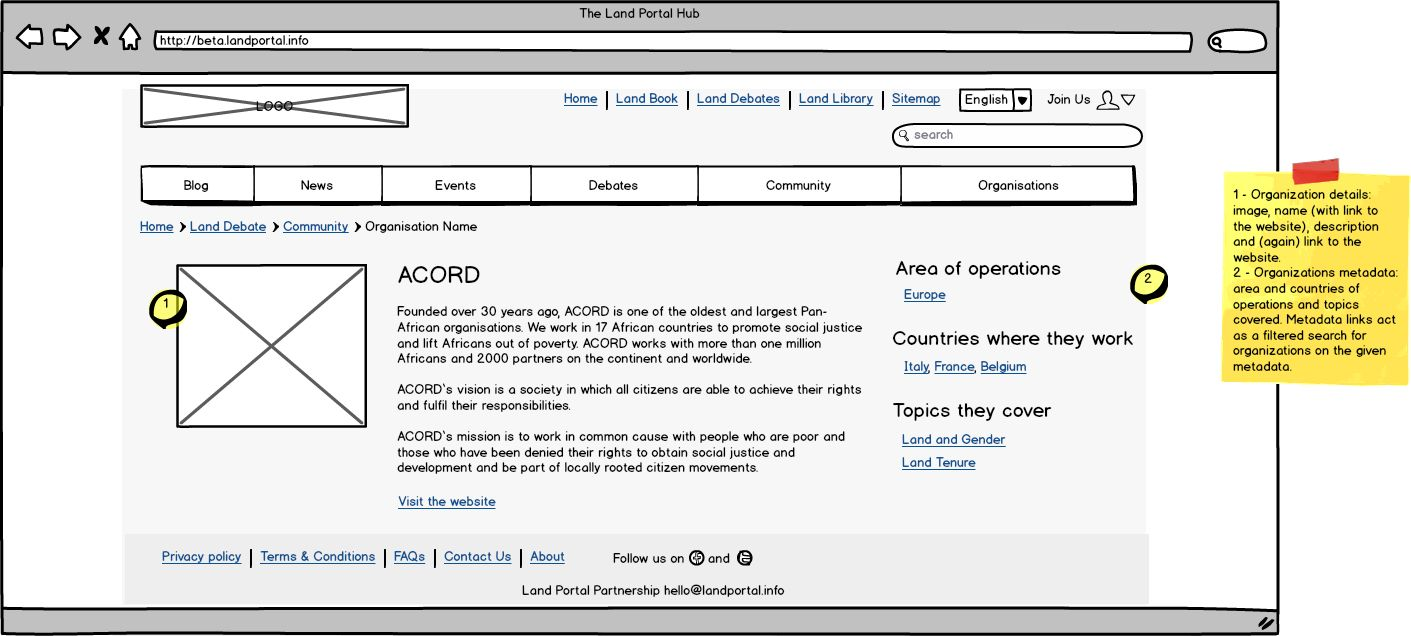
\includegraphics[width=\textwidth]{mockups/organisation}
	\caption{\textit{Mockup} de la vista de detalle de una organización}
	\label{fig:mockup_organizacion}
\end{figure}


\subsubsection{Vista de comunidad}
La vista de la comunidad será similar a la vista de organizaciones, la cual se puede ver en la figura \ref{fig:mockup_organizaciones}.  Las únicas diferencias respecto a la vista de organizaciónes serán:
\begin{itemize}
	\item En lugar de mostrar las organizaciones del portal, esta vista mostrará en una parrilla o \textit{grid} los usuarios registrados en el portal.
	\item En la zona derecha (además del formulario de búsqueda y el \textit{widget} de la red social Facebook) se incluirá un botón para facilitar el registro de nuevos usuarios.
\end{itemize}

\subsubsection{Vista de login}
La figura \ref{fig:mockup_login} muestra el \textit{mockup} de la vista de login. Esta vista permitirá que los usuarios inicien sesión en el portal.  La vista de login contará con un formulario donde el usuario introducirá su nombre de usuario o email y su contraseña para iniciar sesión en el sistema.  También existirá un enlace mediante el cual un usuario podrá solicitar una nueva contraseña en caso de haber olvidado la suya.

Además, siguiendo con la línea social del portal, se incluyen dos botones destinados a iniciar sesión en el sistema utilizando las redes sociales Twitter y Facebook.

\begin{figure}[h]
	\centering
	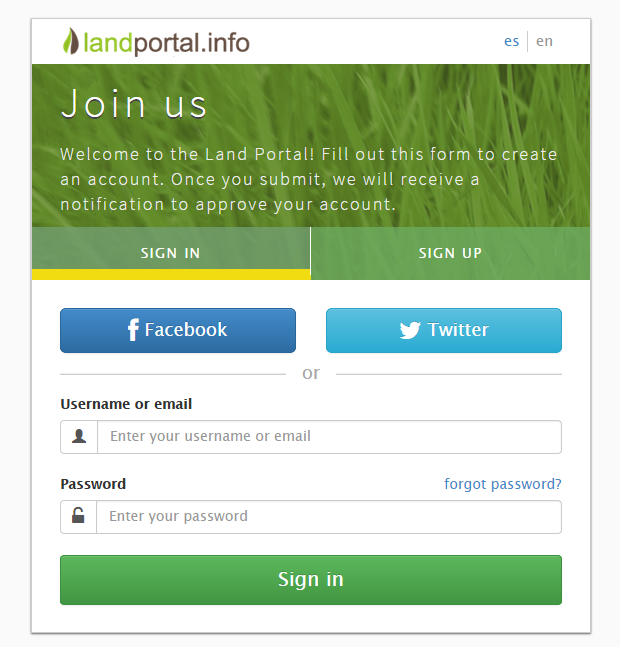
\includegraphics[width=\textwidth]{mockups/login}
	\caption{\textit{Mockup} de la vista de login}
	\label{fig:mockup_login}
\end{figure}


\subsubsection{Vista de registro}
La figura \ref{fig:mockup_registro} muestra el \textit{mockup} de la vista de registro. Esta vista permitirá a los usuarios crear una nueva cuenta en el sistema.  La vista de registro contará con un formulario donde el usuario introducirá su nombre de usuario, su email, su nombre y apellidos y los países y continentes en los que esté interesado. Los campos obligatorios para crear una nueva cuenta de usuario están marcados con un asterisco.  

El botón de registro creará la nueva cuenta en el sistema con un estado ``desactivado'', a la espera de ser activada por un administrador.

\begin{figure}[h]
	\centering
	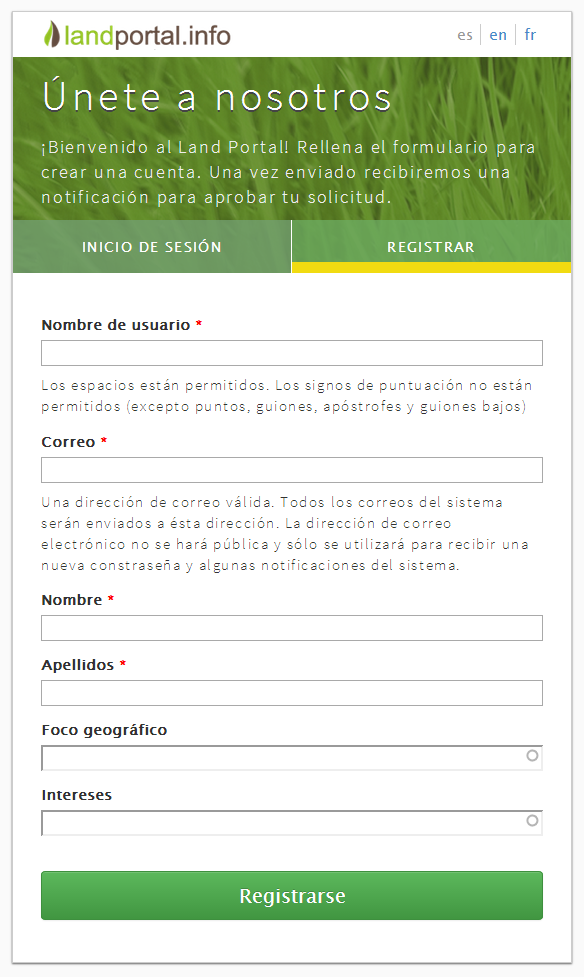
\includegraphics[width=\textwidth]{mockups/register}
	\caption{\textit{Mockup} de la vista de registro}
	\label{fig:mockup_registro}
\end{figure}




\subsubsection{Vista de búsqueda}
La figura \ref{fig:mockup_buscar} muestra el \textit{mockup} de la vista de búsqueda.  Esta vista permitirá a los usuarios buscar cualquier tipo de contenido en el portal.   Al pulsar sobre cada resultado de búsqueda el usuario accederá a la vista de detalle del mismo.

Como se puede ver en la imagen, cada resultado de la búsqueda se presentará de una forma diferente y tendrá asociada una etiqueta en la que se indica el tipo de contenido al que pertenece.  Al pulsar en esta etiqueta, el sistema cargará la vista correspondiente a cada tipo de contenido.

\begin{figure}[h]
	\centering
	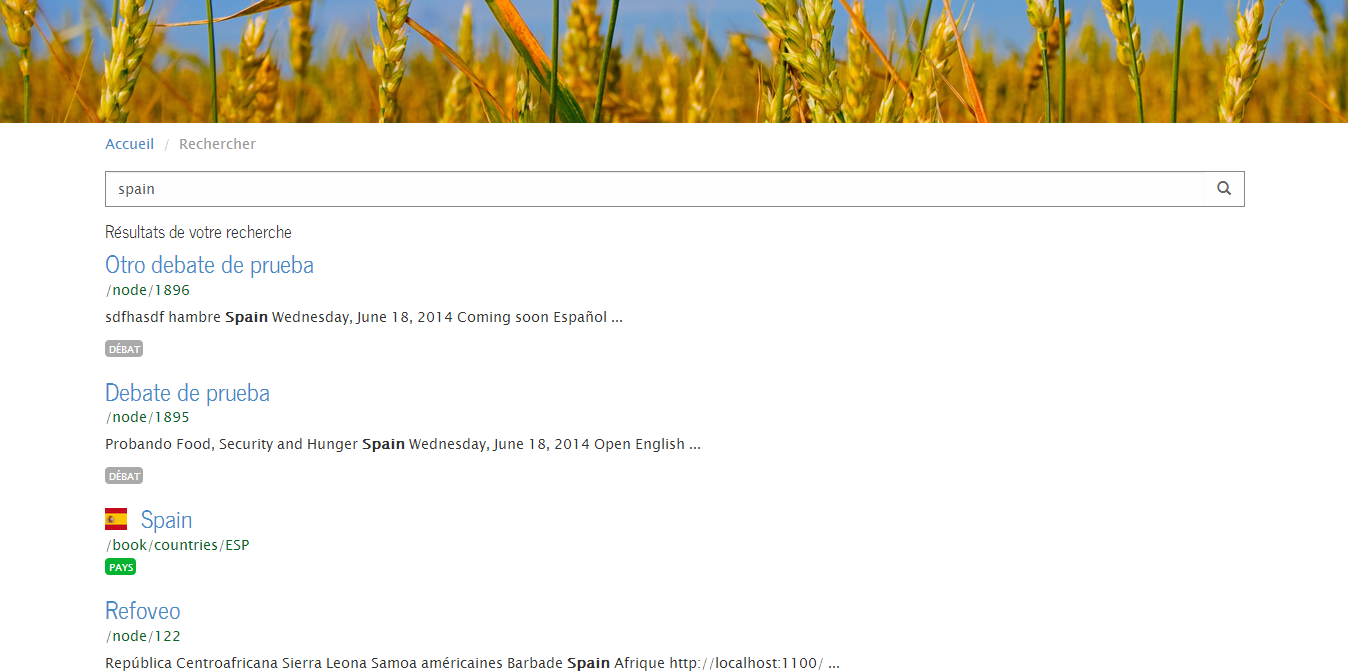
\includegraphics[width=\textwidth]{mockups/search}
	\caption{\textit{Mockup} de la vista de busqueda}
	\label{fig:mockup_buscar}
\end{figure}